% \section{Computation, dynamics and symmetry}



% %%%%%%%%%%%%%%%%%%%%%%%%%%%%%%%%%%%%%%%%%%%%%%%%%%%%%%%%%%
% % \begin{frame}[label=ladila]{The criticality view I}
% %  \begin{center}
% %   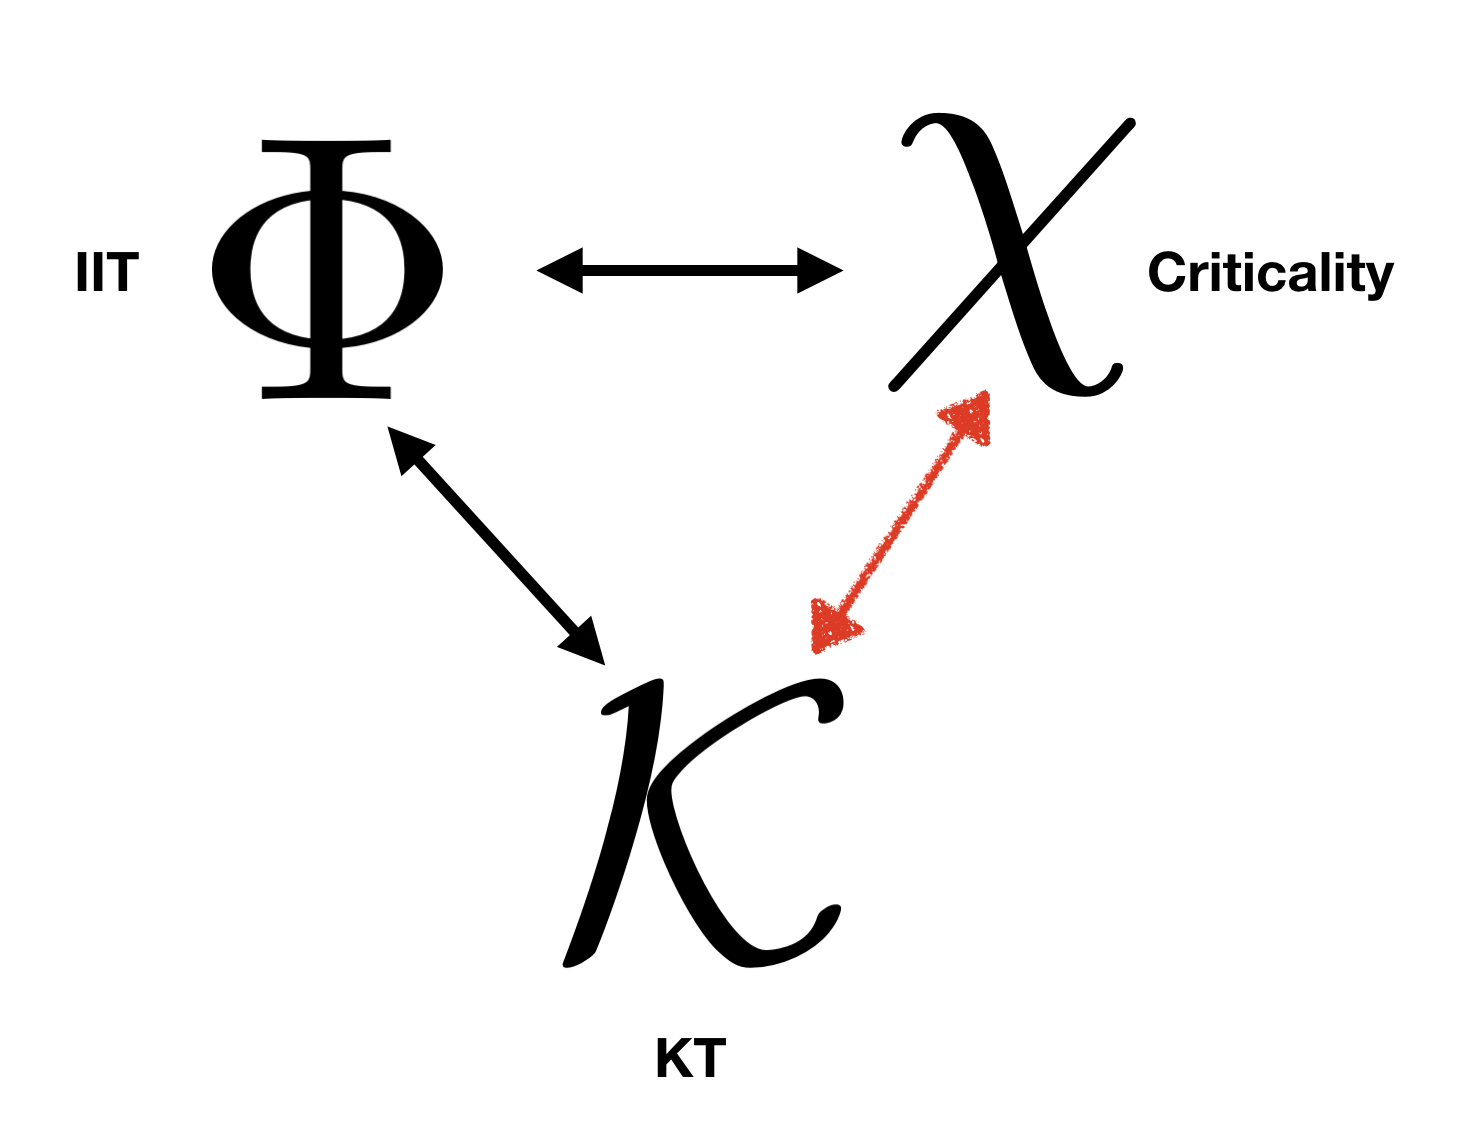
\includegraphics[height=8cm]{img/KUF.png}
% %   \end{center}
% % \end{frame}


% %%%%%%%%%%%%%%%%%%%%%%%%%%%%%%%%%%%%%%%%%%%%%%%%%%%%%%%%%%
% % \begin{frame}[label=ladila]{Towards computational neurophenomenology}
% %  \textbf{Computation} in Nature is carried out by dynamical systems with very large degrees of freedom.  \vfill
 
% %   To compute, brains operate close (but above)  to the boundary of  \textbf{critical transitions}  \citep{Bak1988,Chialvo:2004aa,Cocchi2017,Carhart2018,Deco2021} $\longrightarrow$maximal information flow, multistability/metastability. \vfill
  
% %   E.g., altered state of consciousness appear to move the brain away from the transition point (e.g., psychedelics towards more disorder) \citep{CarhartHarris2019,Ruffini:2022ac}. %Ising temperature under LSD increases (Ruffini et al in prep).  
% %   \vfill
  
% %   Algorithmic agents (dynamical systems instantiating  compressive models of  algorithmically generated data)  must have other special properties. In particular, \vfill
  
% %   \textbf{How can we characterize the structure in models?} This should match the phenomenological structure of experience (\SEP).\vfill

% %  %For example, we can show that \textit{agent dynamics must lie in a reduced manifold}.
% %   \end{frame}
  
  
% % \begin{frame}[label=st] {Characterizing models}
    
% %      How can we \textbf{define model structure?} Measure it? \vfill
     
% %      In a recent paper\cite{ruffiniStructuredDynamicsAlgorithmic2023}, we first \textbf{define generative models using group theory}, capturing the idea of simplicity as symmetry. Then, we show that:
% %     \vfill
% %    % We associate the algorithmic simplicity of a model with representations of Lie groups or Lie algebras with special properties such as nilpotency and compositionality (hierarchical function composition).
   
% %  % 1)  Neural networks, such as FFNs, inherit \textbf{structural constraints} from the symmetry properties of the data on which they are trained.\vfill
    
% %      %We discuss the role of symmetry, conservation laws, and compatible \textbf{world-tracking constraints}.
    
% %     1) Tracking the world forces the agent as a dynamical system to mirror the symmetry in the data.\textbf{ Dynamics collapses to reduced manifolds}. \vfill
    
% %     2) The hierarchical nature of world data leads to coarse-graining and the notion of \textbf{hierarchical constraints and manifolds}.\vfill
    
% % \end{frame}


% %%%%%%%%%%%%%%%%%%%%%%%%%%%%%%%%%%%%%%%%%%%%%%%%%%%%%%%%%%
% %   \begin{frame}[label=ladila]{The criticality view III}
% %   Recall the movie of a moving hand in empty space, $y(t) = f(\theta(t))$. %, where $y(t)$ represents the sequences of images of the hand as a function of parameters $\theta(t)$.
% %   \vfill
  
% %   Although $y$ may be embedded in a very high dimensional space, its dimension is actually very small if the set of parameters $\theta$ controlling the hand function is small.\vfill
  
% % The state of a dynamical system generating frames of the moving hand, regardless of how large its natural space is  (e.g.,   large number of neurons) must also lie in a low dimensional subspace, a {\bf reduced manifold}. How?  \vfill
  
% %    Criticality: near criticality (Re[$\lambda$]$\sim0$) the dynamics of complex systems collapse to low dimensional manifolds   \citep{Jirsa2020,Jirsa2022}---constrained dynamics. \vfill
   
% %    Symmetry: in a Hamiltonian dynamical system where $g = y(t)-f(\theta(t)) = 0$  (the constraint),  Noether's theorem states that  $H$ is invariant under the group of symmetries generated by $g$  \citep{Dirac2001-gi,Jose1998-qy}). 

% % \end{frame}

% % %%%%%%%%%%%%%%%%%%%%%%%%%%%%%%%%%%%%%%%%%%%%%%%%%%%%%%%%%%
% % \begin{frame}[label=ladila]{The criticality view IV---the center manifold}
% % Trajectory of representation of hand in reduced manifold. 
% %  \begin{center}
% %   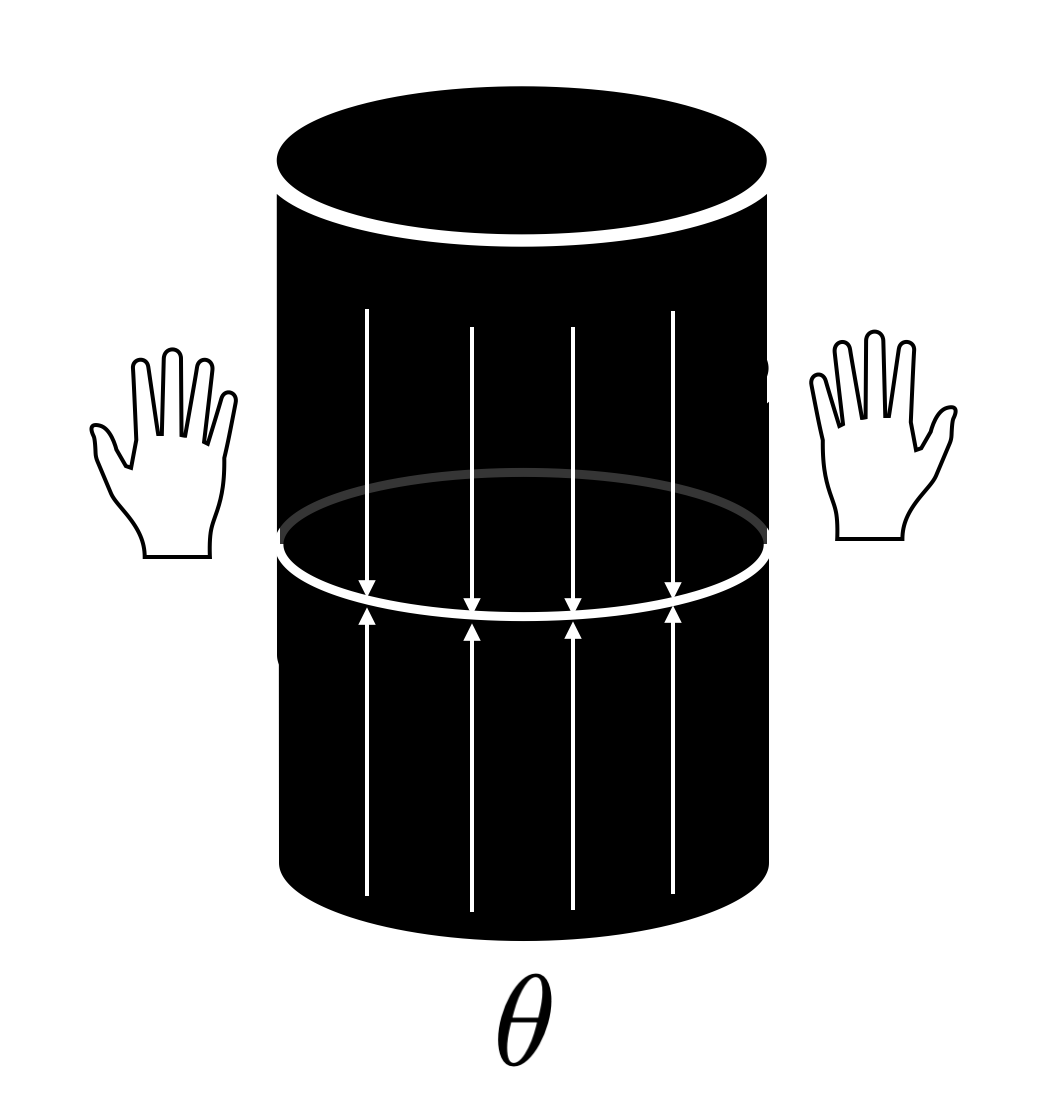
\includegraphics[height=6cm]{img/cylinder.png}
% %   \end{center}


% % \end{frame}




% % The agent must continuously verify whether its internal models accurately reflect the external world. This verification occurs at the Comparator, a mechanism where the agent compares incoming real-world data with the data generated by its model (predictions). Mathematically, this process can be described as imposing a “world-tracking constraint” on the system. In simple terms, this constraint ensures that the output or readout from the model aligns with the actual input data received from the world.

% % When we introduce this constraint to the ordinary differential equations (ODEs) governing the model’s dynamics, it effectively imposes a set of symmetry properties on the ODE. These symmetries reflect the underlying regularities or simplicity of the world’s generation process. In other words, by constraining the model to track the world accurately, the system must respect certain symmetries or patterns that arise from the structure of the external world itself. This leads to a model that not only fits the data but also incorporates the inherent simplicity or regularity of the processes generating that data.

% % Breakdown:

% % 	1.	Comparator: The agent checks if its model’s predictions match the incoming data.
% % 	2.	World-Tracking Constraint: This mathematical constraint enforces a requirement that the model’s internal state reflects the real-world data.
% % 	3.	Symmetry in the ODE: The constraint on the ODE forces it to obey certain symmetry properties, which mirror the simplicity or regularities of the world.{The world-tracking condition enforces symmetry}

% \begin{frame}{1. The world-tracking equations (mathematics of Comparator)}
% Consider an agent tracking  data $I_{\theta}$ (visual) generated by a simple world model --- a hand, say. A group ``moves'' the hand through $\theta$. \vfill

% \begin{minipage}{0.5\linewidth}
%     The world-tracking equations of the agent as a dynamical system are
%     \begin{eqnarray*}\label{eq:WTNE} 
%         \dot x &=& f\big(x; w, I_{\theta}\big) \nonumber \\
%         g(x)  &\approx &I_{\theta}
%     \end{eqnarray*}
%     i.e., an ODE plus a constraint. They must hold for all values of $\theta$ (all hand images).
% \end{minipage}%
% \hfill
% \begin{minipage}{0.45\linewidth}
%     \centering
%     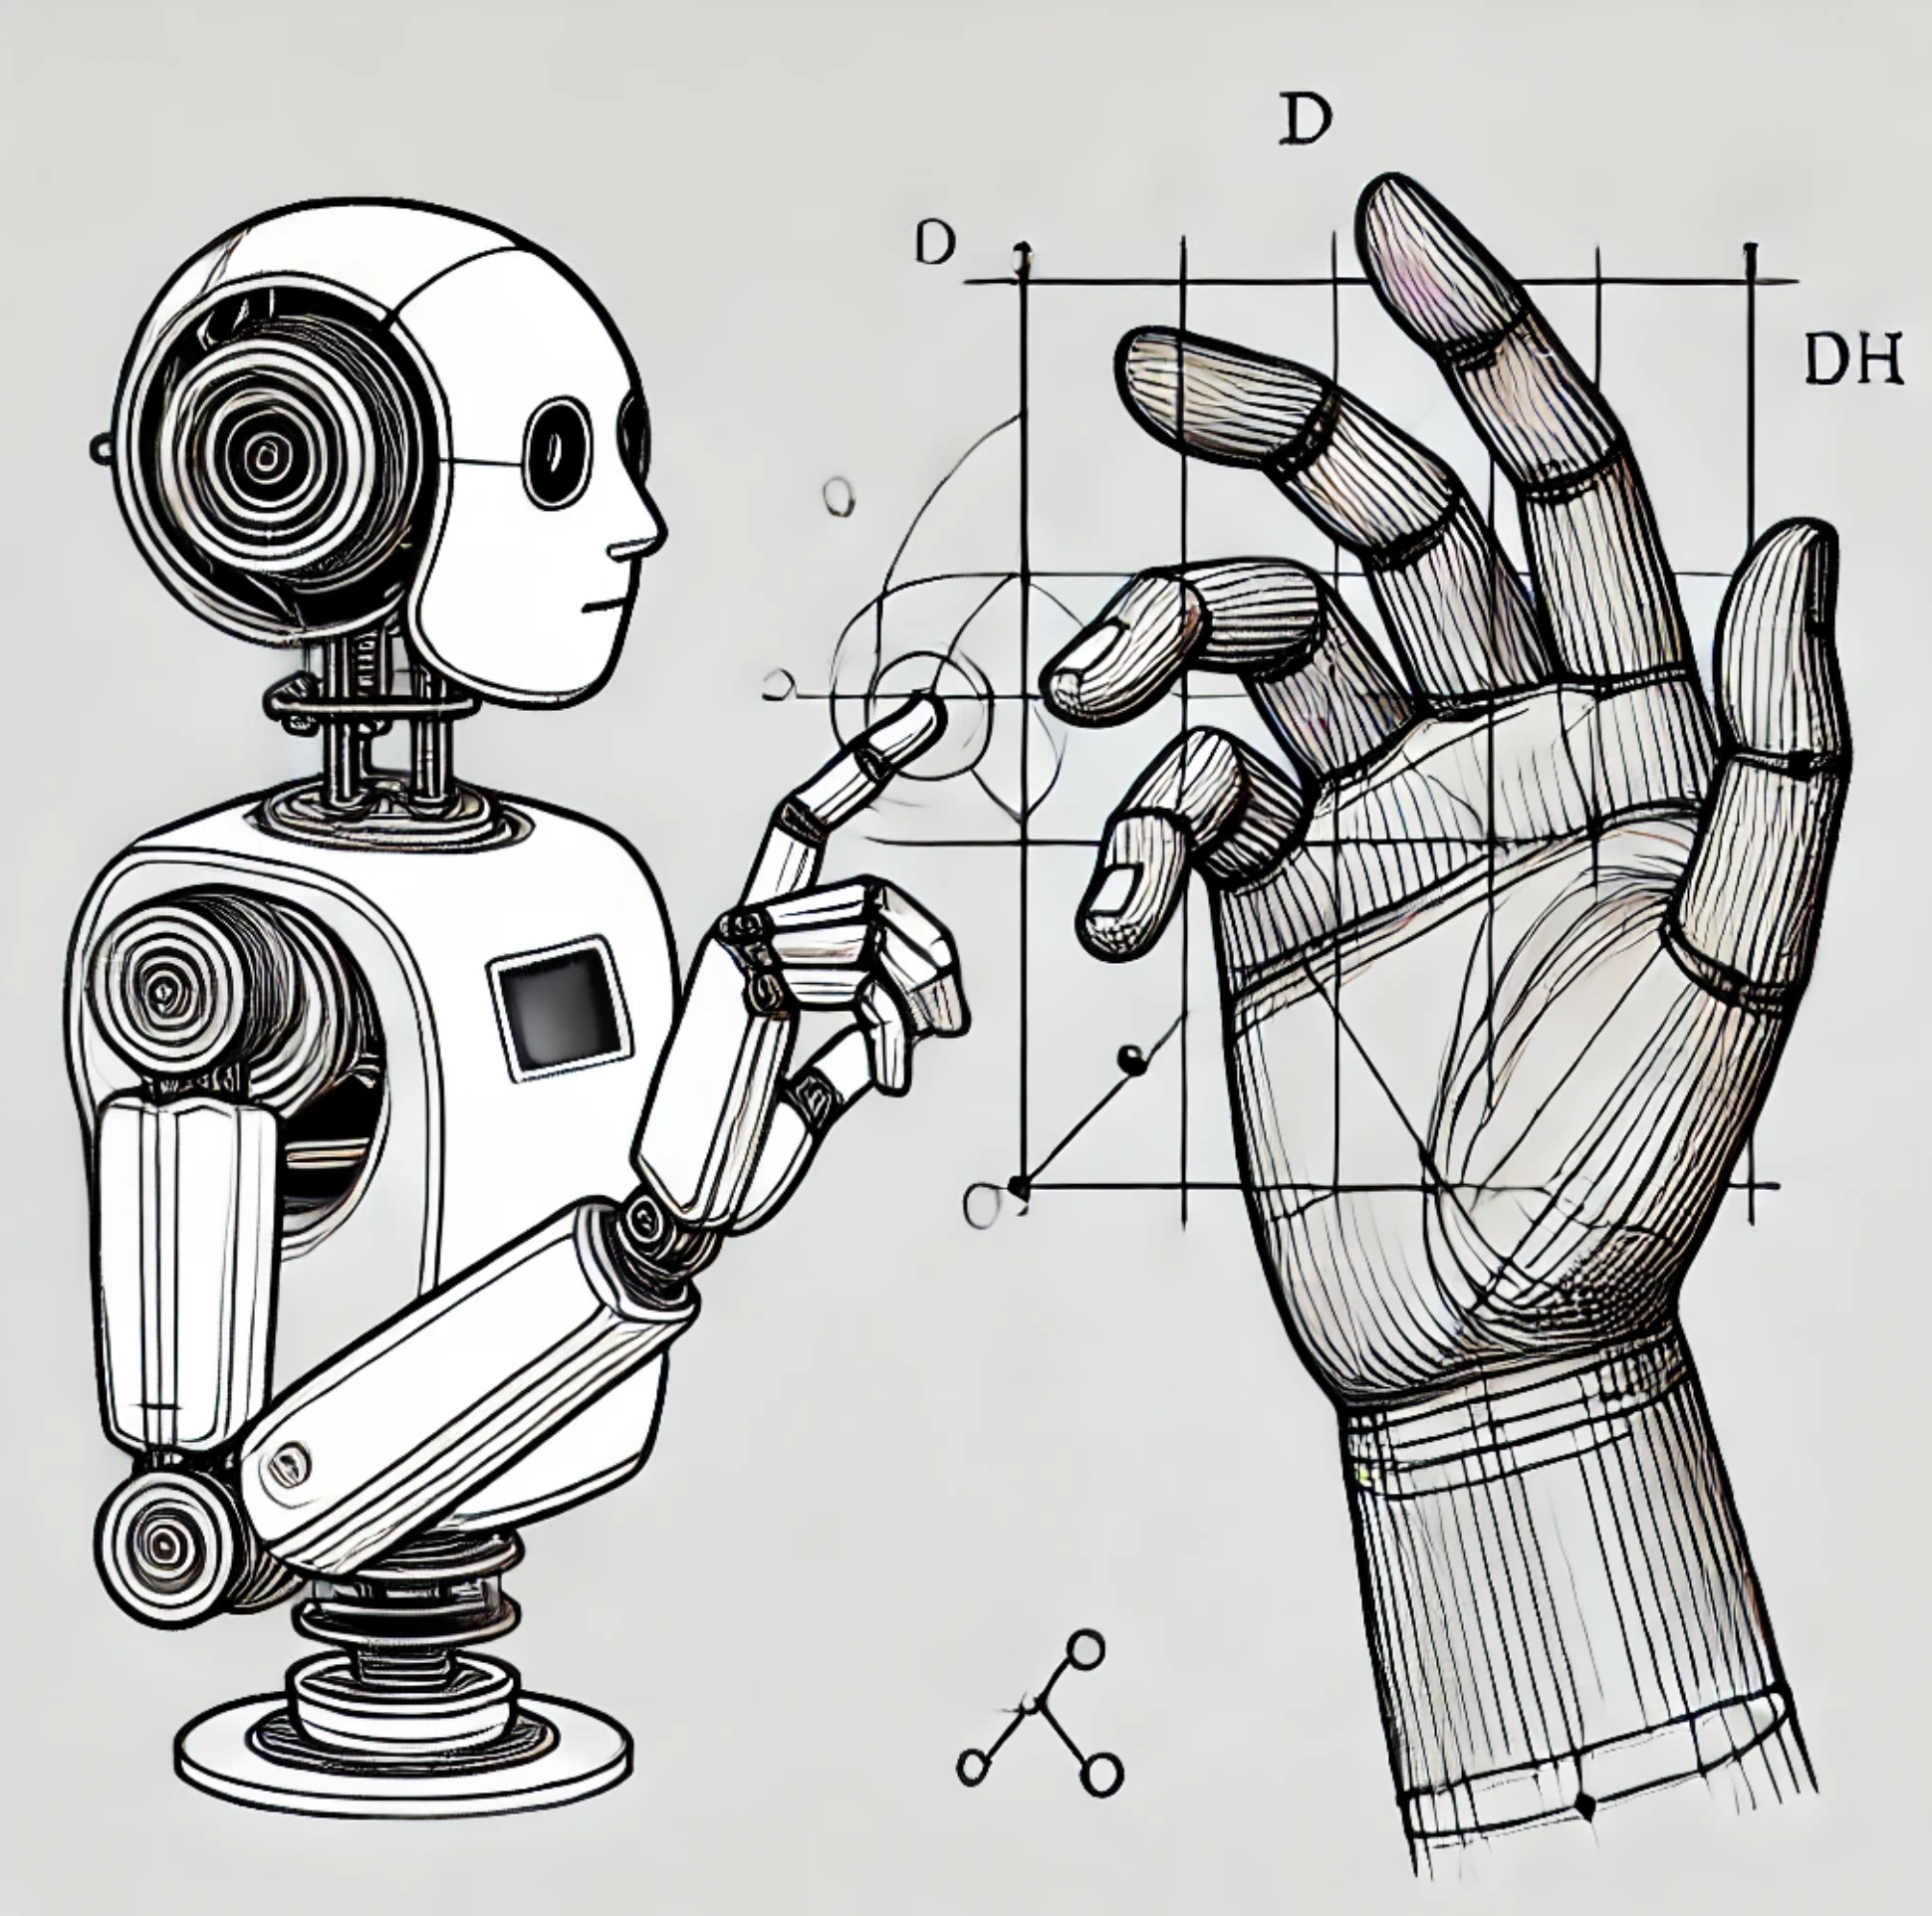
\includegraphics[width=0.6\linewidth]{hand.png}
% \end{minipage}
% \begin{tcolorbox}[colback=cyan!40, colframe=gray!70,  title={Connecting dynamics and symmetry}]  
% To satisfy these,  \textbf{the ODEs must exhibit symmetry} $\Rightarrow$ conservation laws. Dynamics collapses to a reduced manifold \cite{ruffiniStructuredDynamicsAlgorithmic2023}. 
% \end{tcolorbox}

% %\vfill
% % \begin{tcolorbox}[colback=gray!10, colframe=gray!70, title={Dynamics and symmetry}]

% %  \end{tcolorbox}

% %This is how the Mutual Algorithmic Information between agent and World manifests in dynamics.
% \end{frame}


% % \begin{frame}{The world-tracking equations (mathematics of \SEP!)}
% % %We assume the agent seeks to track (match) data $I_{\theta (t)}$ generated by a simple world model --- a hand, say. A Lie group ``moves'' the hand. \vfill

% % \begin{minipage}{0.4\linewidth}
% %     Separate $x$ as $z$ (internal) and (readout) $u=g(z) \equiv w_u x$. \vspace{0.5cm}
    
% %     The equations %of the agent as a dynamical system 
% %     become
% %     \begin{eqnarray*}\label{eq:WTNE} 
% %         \dot z &=& f\big(z; w, I_{\theta(t)}\big) \nonumber \\
% %         u  &\approx &I_{\theta (t)}
% %     \end{eqnarray*}
% % \end{minipage}%
% % \hfill
% % \begin{minipage}{0.60\linewidth}
% %     \centering
% %        % 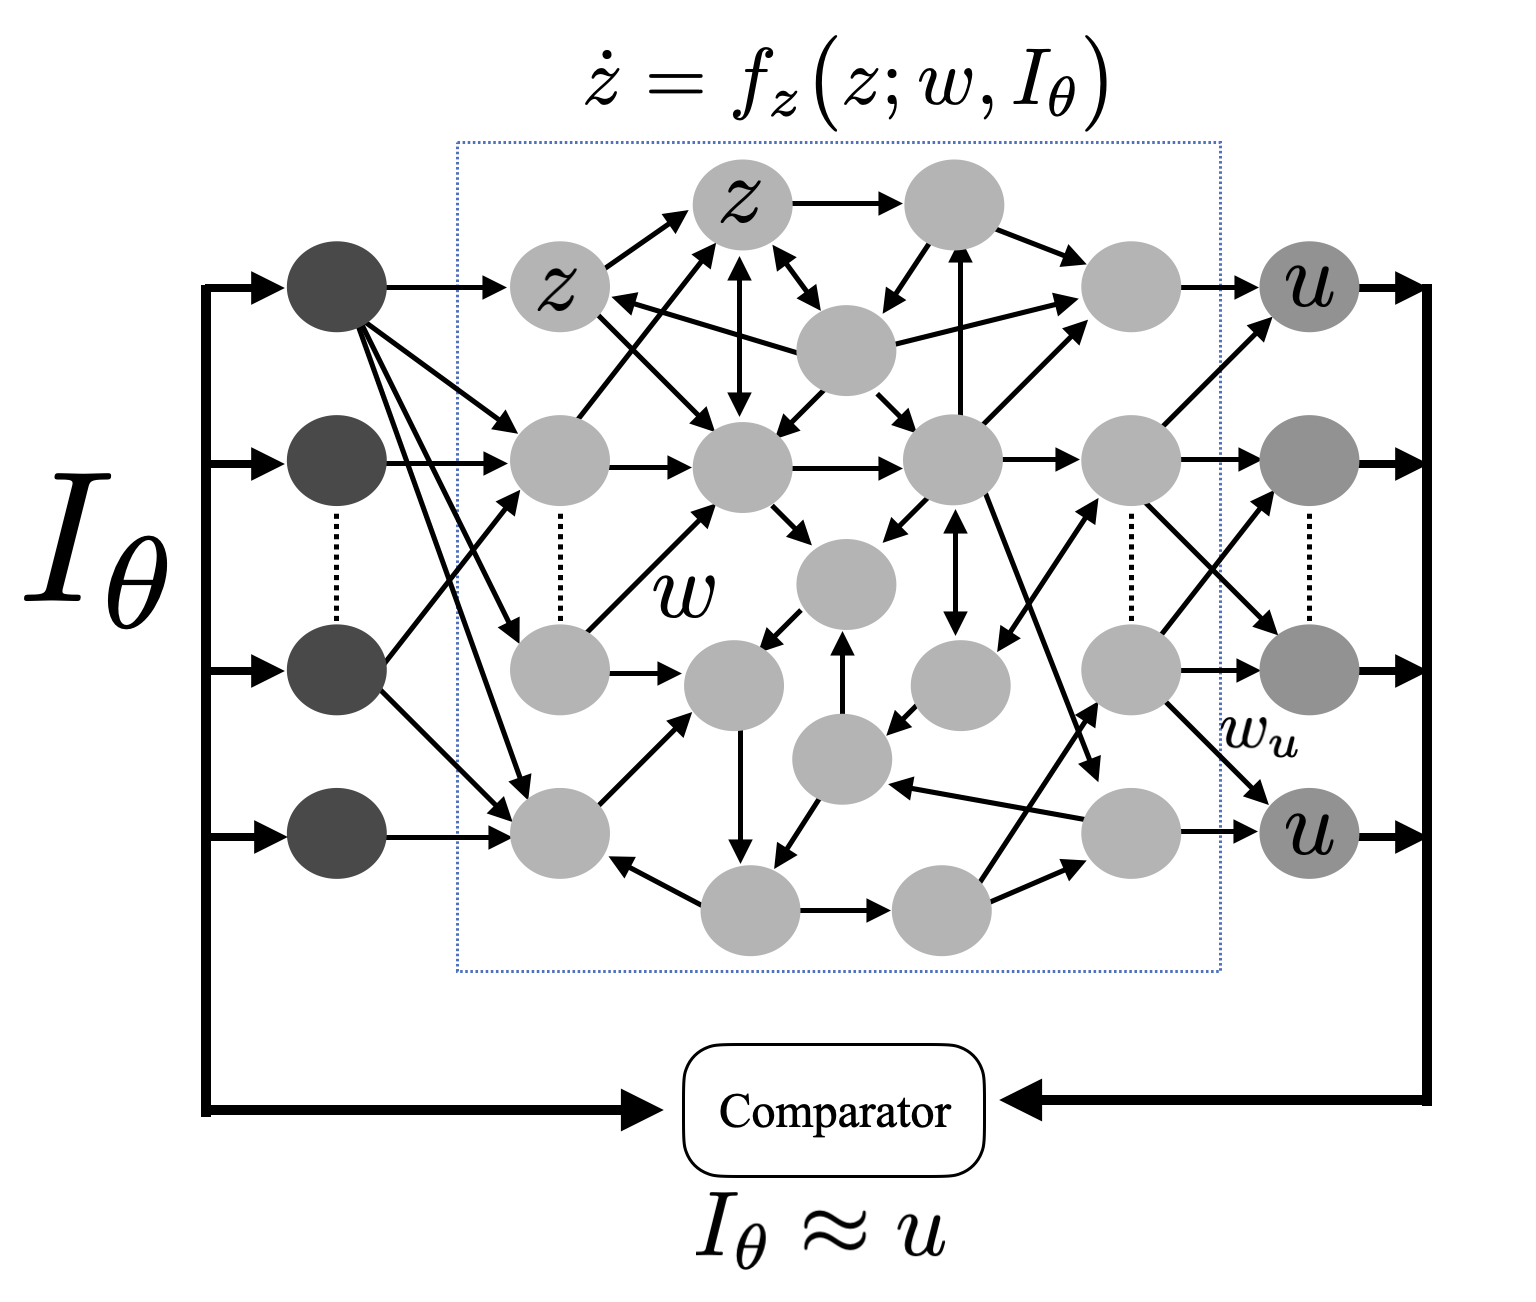
\includegraphics[width=0.9\linewidth]{wt.png}


% %     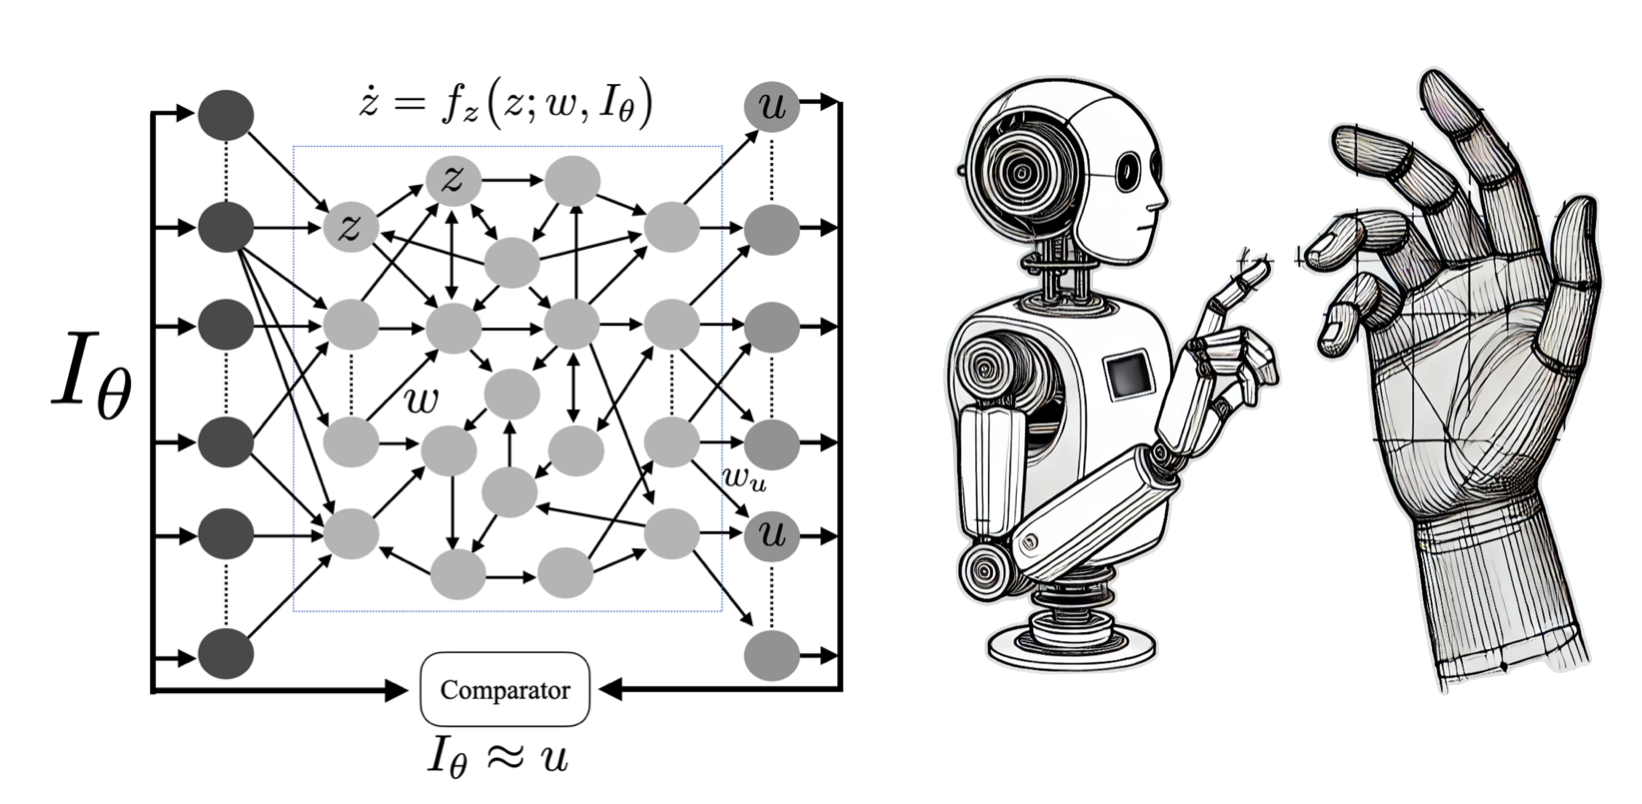
\includegraphics[width=1\linewidth]{handnetwork.png}

% % \end{minipage}

% % \vfill



% % \begin{tcolorbox}[colback=gray!10, colframe=gray!70, title={Connecting MAI, dynamics and symmetry}]
% % %To satisfy them, one can show that \textbf{the ODEs must possess symmetry}\cite{ruffiniStructuredDynamicsAlgorithmic2023}.  
% % Through \textbf{shared symmetry}, the  \textbf{Mutual Algorithmic Information} between the agent and the World manifests in dynamics.
% % \end{tcolorbox}
% % \end{frame}

% %  \begin{frame}{The world-tracking equations (mathematics of \SEP!)}
% % %We assume the agent seeks to track (match) data $I_{\theta (t)}$ generated by a simple world model --- a hand, say. A Lie group ``moves'' the hand. \vfill

% % % \begin{minipage}{0.4\linewidth}
% % %     Separating $x$ as $z$ (internal) and  $u=g(z) \equiv w_u x$ (readout), \vspace{0.25cm}
    
% % %     %The equations %of the agent as a dynamical system 
% % %     %become
% % %     \begin{eqnarray*}\label{eq:WTNE} 
% % %         \dot z &=& f\big(z; w, I_{\theta(t)}\big) \nonumber \\
% % %         u  &\approx &I_{\theta (t)}
% % %     \end{eqnarray*}
% % % \end{minipage}%
% % % \hfill
% % % \begin{minipage}{0.60\linewidth}
% % %     \centering
% % %        % 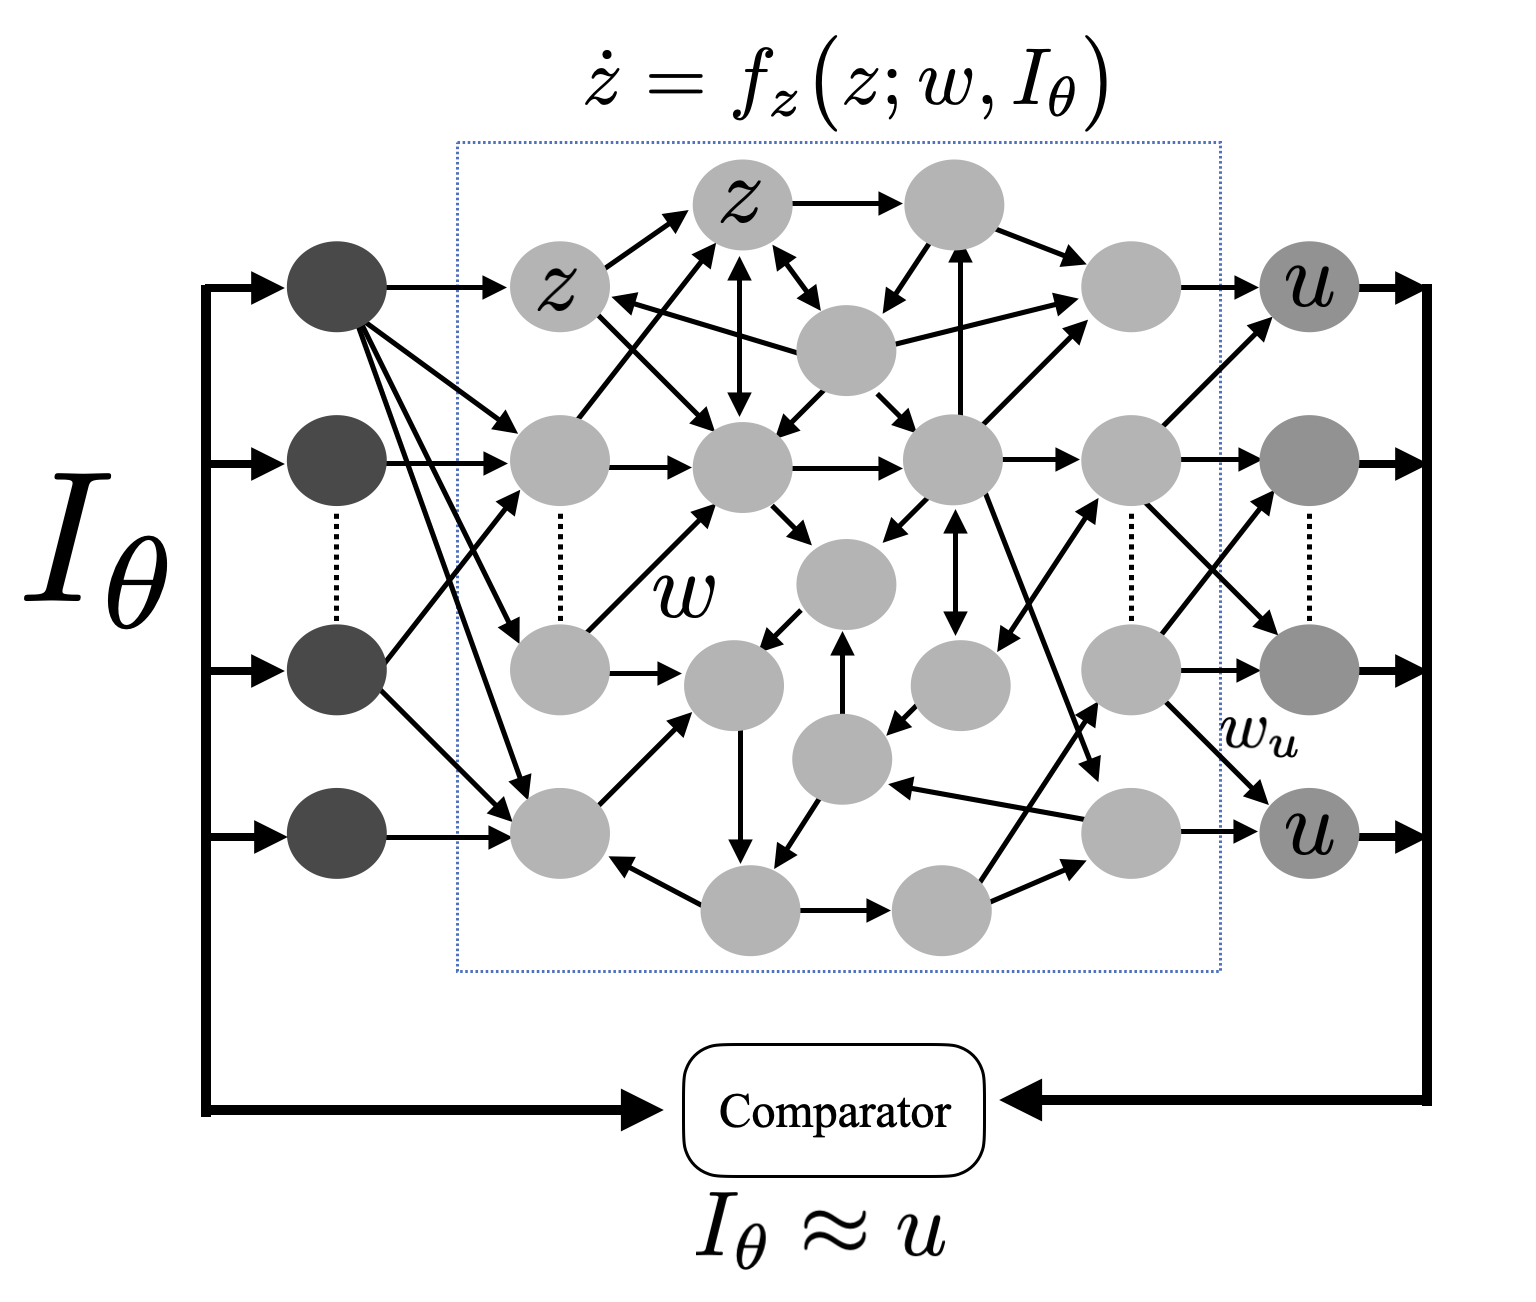
\includegraphics[width=0.9\linewidth]{wt.png}


% % %     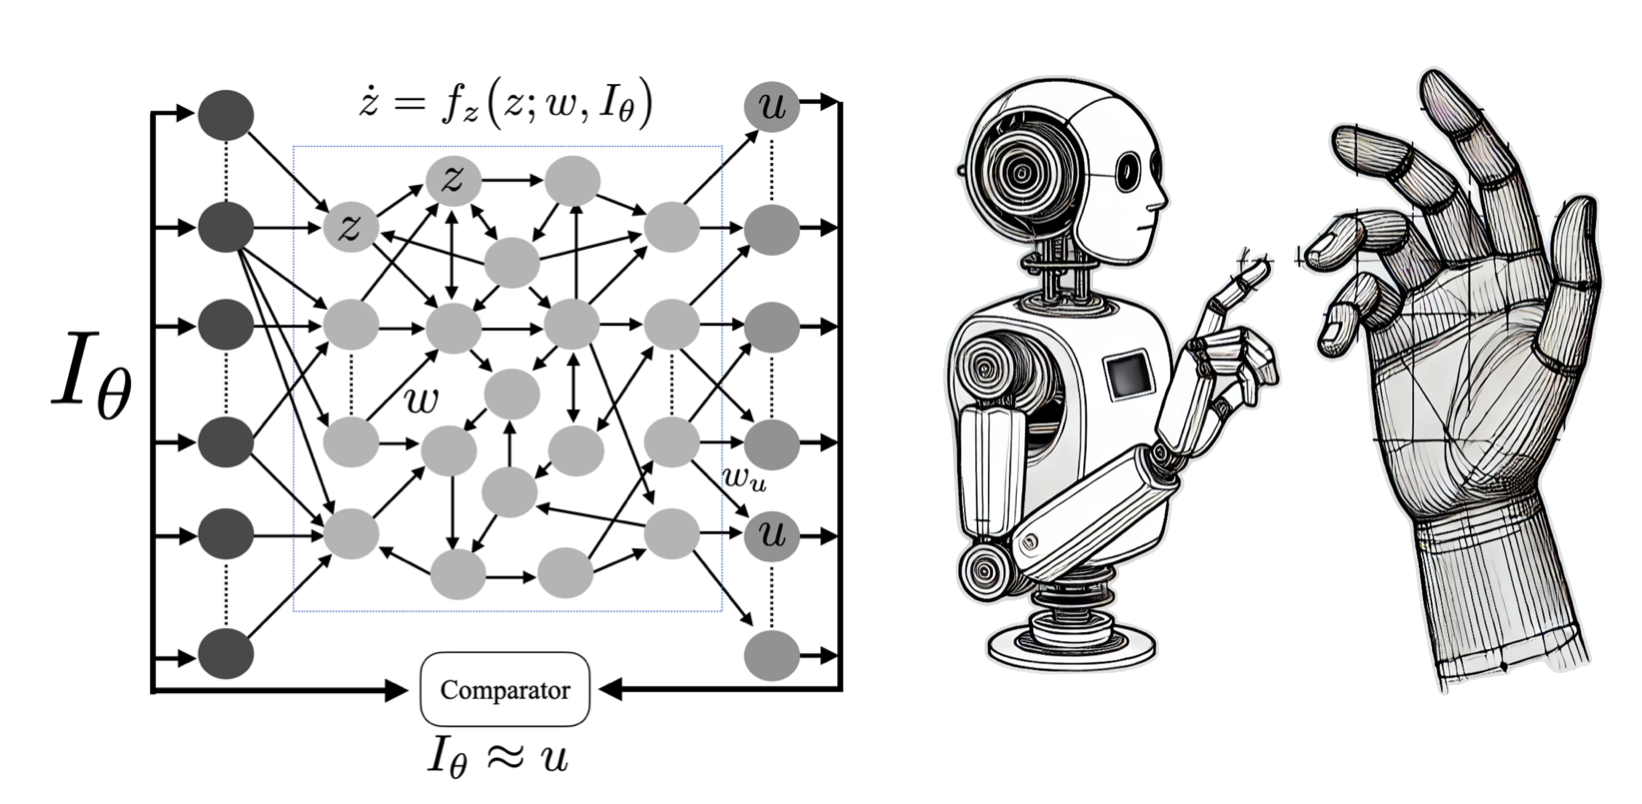
\includegraphics[width=1\linewidth]{handnetwork.png}

% % % \end{minipage}

% % % \vfill

% %   \centering
% %        % 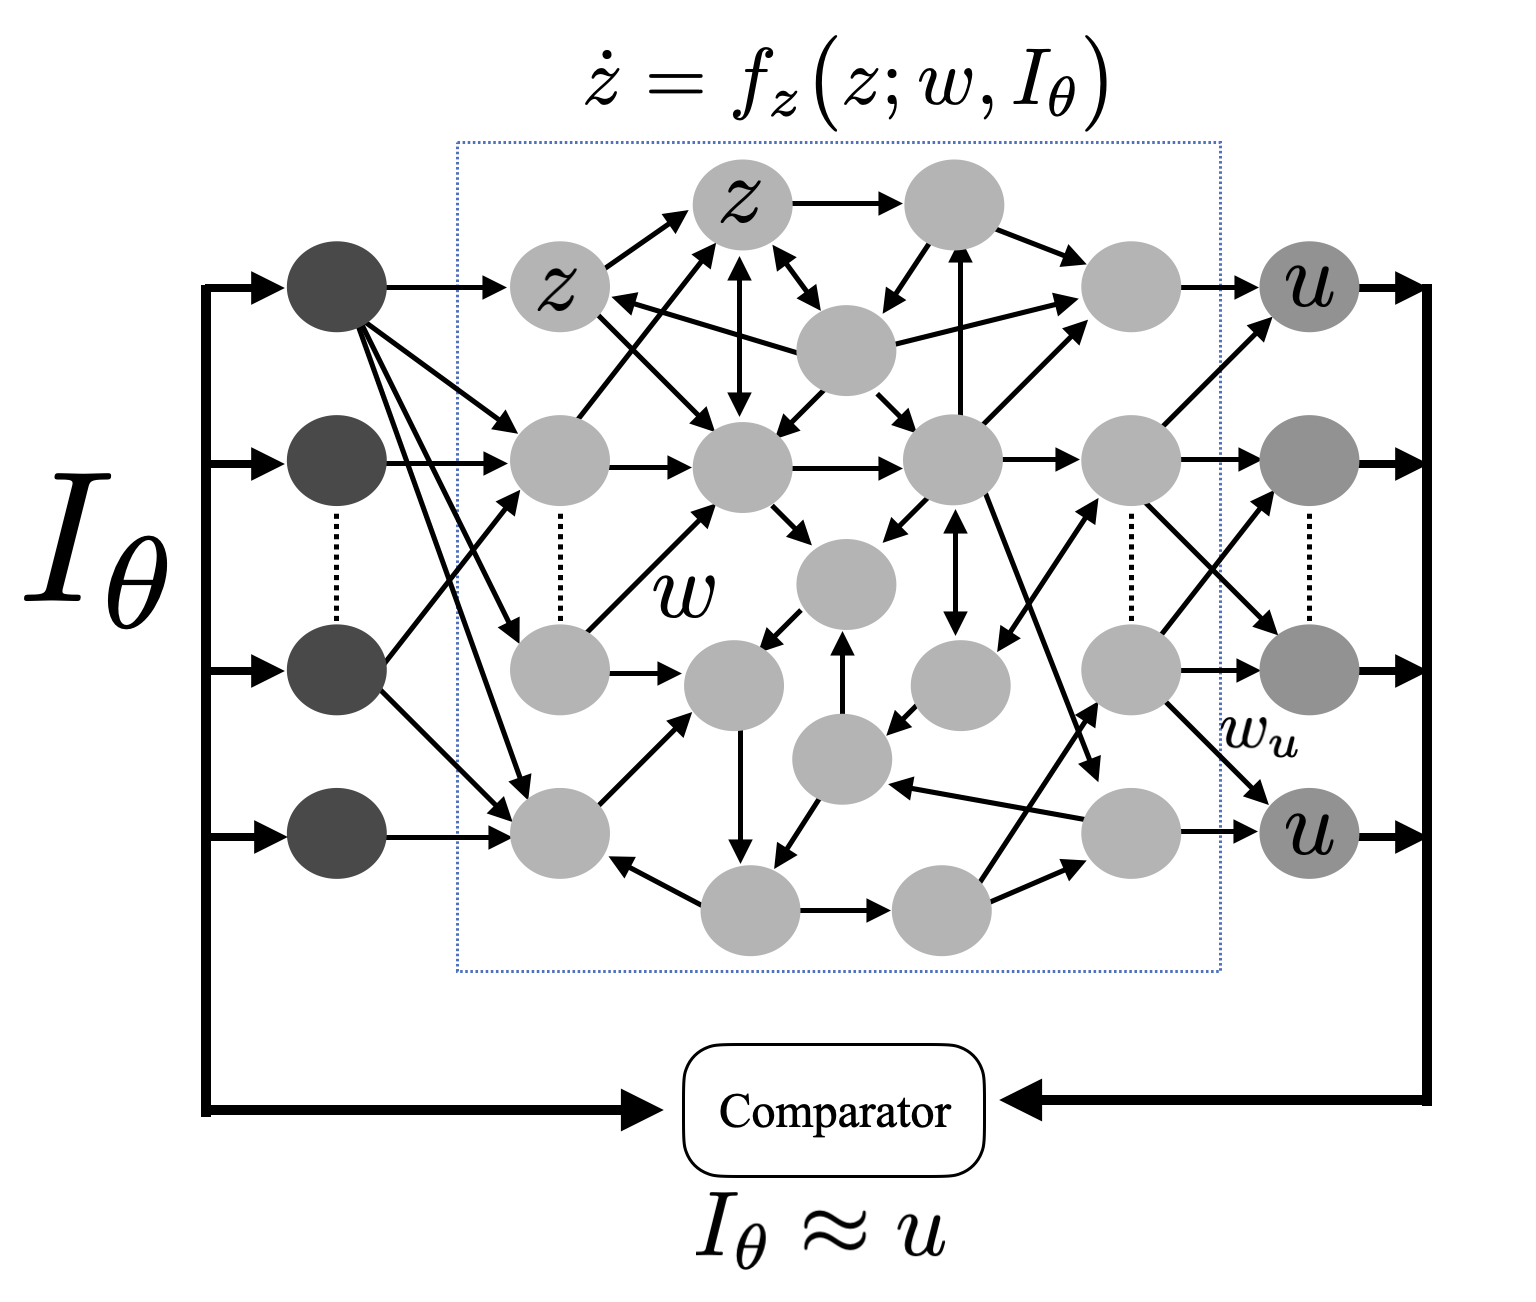
\includegraphics[width=0.9\linewidth]{wt.png}


% %     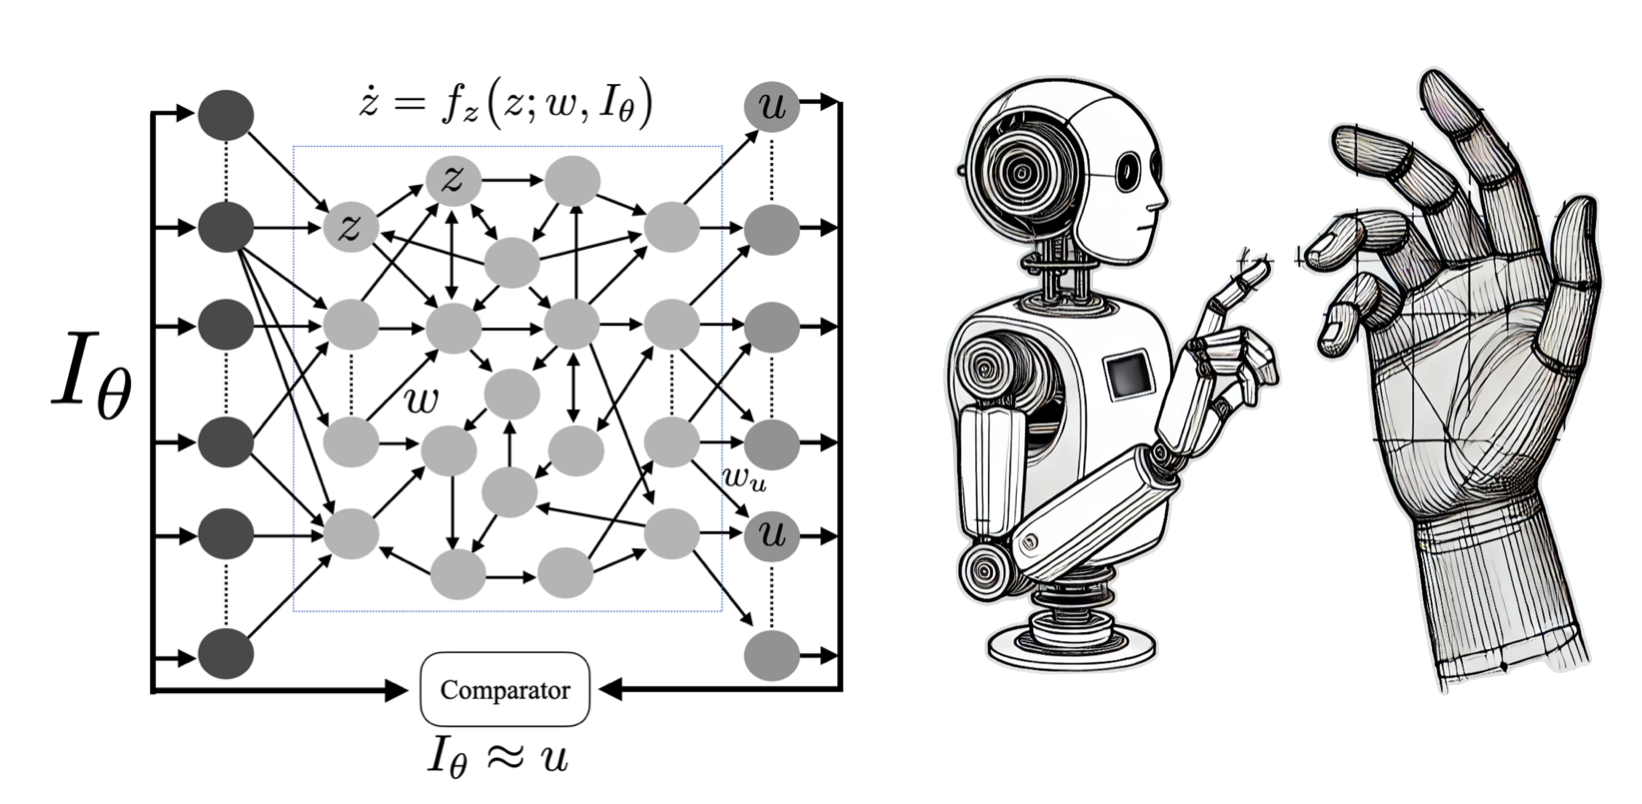
\includegraphics[width=0.6\linewidth]{handnetwork.png}
    

% % \begin{tcolorbox}[colback=cyan!40, colframe=gray!70,  title={Connecting MAI, dynamics and symmetry}]
% % %To satisfy them, one can show that \textbf{the ODEs must possess symmetry}\cite{ruffiniStructuredDynamicsAlgorithmic2023}.  
% % %To satisfy these equations,  \textbf{the ODEs must possess symmetry} \cite{ruffiniStructuredDynamicsAlgorithmic2023}. 

% % Through \textbf{shared symmetry}, the  \textbf{Mutual Algorithmic Information} between the agent and the world manifests in dynamics.
% % \end{tcolorbox}
% % \end{frame}




% %%%%%%%%%%%%%%%%%%%%%%%%%%%%%%%%%%%%%%%%%%%%%%%%%%%%%%%%%%

% %%%%%%%%%%%%%

% \begin{frame}{2. Hierarchical Constraints and Manifolds\cite{ruffiniStructuredDynamicsAlgorithmic2023}}
%     \begin{itemize}
%         \item \textbf{Hierarchical coarse-graining}:
%         \begin{itemize}
%             \item Modeling, planning, and objective function evaluation are inherently \textbf{hierarchical}, arising from the compositional nature of real-world data.
%             \item Resource-limited agents employ (lossy) \textbf{coarse-graining} to compress data in useful  ways \cite{ruffiniNavigatingComplexityHow2024} (spatiotemporal averaging, dimensionality reduction techniques...)
%         % \end{itemize}
%         % \item \textbf{Hierarchical coarse-graining in the brain}:
%         % \begin{itemize}
%             \item The brain processes information through\textbf{ hierarchical coarse-graining}, aggregating details to form higher-level representations in visual and auditory systems \cite{dicarloHowDoesBrain2012,grill-spectorFunctionalArchitectureVentral2014,bizleyWhatWhereHow2013}.
%         \end{itemize}
%          \vfill
%         \item \textbf{Multilevel World-Tracking Constraints $\longrightarrow$ Hierarchical reduced manifold}:
%         \begin{itemize}
%             \item Constraints at different levels correspond to different scales of coarse-graining.
%             \item Lower-level constraints must be compatible with higher-level constraints, leading to nested structures.
%         \end{itemize}
%     \end{itemize}

% \end{frame}

% % \begin{frame}{Formalizing Nested Coarse-Graining and Hierarchical Constraints}
% %     \textbf{Nested Coarse-Graining Operators}:
% %     \begin{equation*}
% %         \begin{aligned}
% %             \mathbf{y}_1 &= \mathcal{G}_1(\mathbf{x}), \\
% %             \mathbf{y}_2 &= \mathcal{G}_2(\mathbf{y}_1), \\
% %             &\ \, \vdots \\
% %             \mathbf{y}_k &= \mathcal{G}_k(\mathbf{y}_{k-1}),
% %         \end{aligned}
% %     \end{equation*}
% %     where:
% %     \begin{itemize}
% %         \item $\mathbf{x} \in \mathbb{R}^n$: Fine-grained state vector.
% %         \item $\mathbf{y}_i \in \mathbb{R}^{n_i}$: Coarse-grained state at level $i$, with $n_i < n_{i-1}$.
% %     \end{itemize}
% %     \textbf{Hierarchical Constraints}:
% %     \begin{equation*}
% %         \mathcal{C}_i(\mathbf{y}_i) = 0
% %     \end{equation*}
% %     \textbf{Constraint Compatibility and Nesting}:
% %     \begin{equation*}
% %         \{\mathbf{y}_{i-1} \mid \mathcal{C}_i(\mathcal{G}_i(\mathbf{y}_{i-1})) = 0\} \subseteq \{\mathbf{y}_{i-1} \mid \mathcal{C}_{i-1}(\mathbf{y}_{i-1}) = 0\}
% %     \end{equation*}

% %     \end{frame}




    

    
% %     \begin{frame}
% %     \textbf{Example}:
% %     \begin{itemize}
% %         \item \textit{High-Level Constraint} ($\mathcal{C}_1$): Recognize the object is a \textbf{cat} $\rightarrow$ Manifold $\mathcal{M}_1$.
% %         \item \textit{Lower-Level Constraint} ($\mathcal{C}_2$): Has \textbf{white fur} and \textbf{blue eyes} $\rightarrow$ Submanifold $\mathcal{M}_2 \subseteq \mathcal{M}_1$.
% %     \end{itemize}

% %     \begin{figure}
% %         \centering
% %         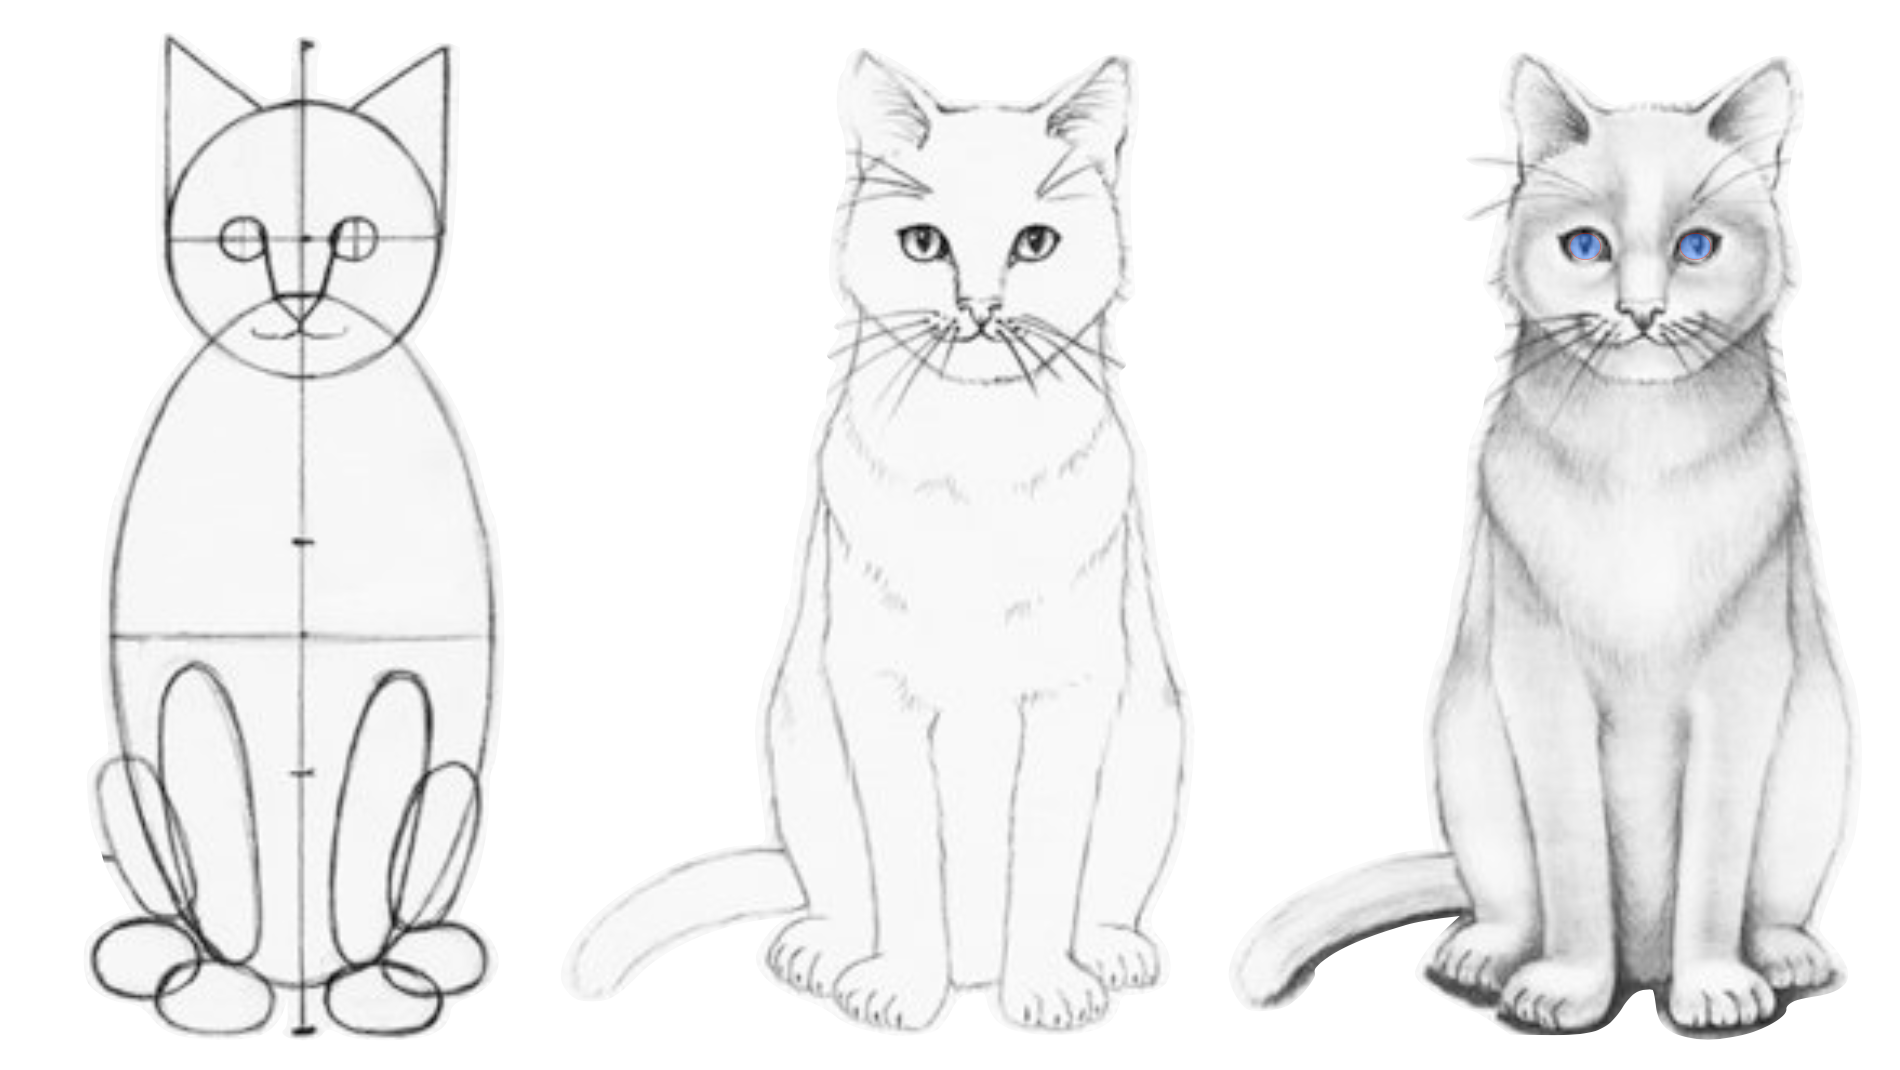
\includegraphics[width=0.5\linewidth]{image10.png}
% %     \end{figure}
% % \end{frame}


% % \begin{frame}{Nested Manifolds}
% %     The constraints generate a sequence,

% %     \begin{equation*}
% %         \mathcal{M}_0 \xrightarrow{\ \mathcal{C}_1\ } \mathcal{M}_1 \xrightarrow{\ \mathcal{C}_2\ } \mathcal{M}_2 \xrightarrow{\ \dots\ } \mathcal{M}_k,
% %     \end{equation*}
% %     where each manifold is defined as:
% %     \begin{equation*}
% %         \mathcal{M}_i = \{\mathbf{y}_{i-1} \in \mathcal{M}_{i-1} \mid \mathcal{C}_i(\mathcal{G}_i(\mathbf{y}_{i-1})) = 0\},
% %     \end{equation*}
% %    % with $\mathcal{M}_0 = \mathbb{R}^n$.

% %         \begin{figure}
% %         \centering
% %         
\includegraphics[width=0.25\linewidth]{image4.png}
% %     \end{figure}
% %     \end{frame}


% % \begin{frame}{Formalizing Nested Coarse-Graining and Hierarchical Constraints}
% %     \textbf{Nested Coarse-Graining Operators}:
% %     \begin{equation*}
% %         \begin{aligned}
% %             \mathbf{y}_1 &= \mathcal{G}_1(\mathbf{x}), \\
% %             \mathbf{y}_2 &= \mathcal{G}_2(\mathbf{y}_1), \\
% %             &\ \, \vdots \\
% %             \mathbf{y}_k &= \mathcal{G}_k(\mathbf{y}_{k-1}),
% %         \end{aligned}
% %     \end{equation*}
% %     where  $\mathbf{x} \in \mathbb{R}^n$ is the finest-grained state vector
% %         and $\mathbf{y}_i \in \mathbb{R}^{n_i}$ the coarse-grained state at level $i$, with $n_i < n_{i-1}$ and $n_0 = n$.
  
% %     \vfill 

    
% % \begin{tcolorbox}[colback=cyan!40, colframe=gray!70, title={The reduced, hierarchical manifold}]
% %     \textbf{Hierarchical Constraints}
% %     $
% %         \mathcal{C}_i(\mathbf{y}_i) = 0
% %     $  generate a sequence, $$\mathcal{M}_0 \xrightarrow{\ \mathcal{C}_1\ } \mathcal{M}_1 \xrightarrow{\ \mathcal{C}_2\ } \mathcal{M}_2 \xrightarrow{\ \dots\ } \mathcal{M}_k$$
% %     \end{tcolorbox}
% % \end{frame}


% % \begin{frame}{Nested Manifolds (multi-level world-tracking conditions)}
% %     The constraints generate a sequence:

% %     \begin{equation*}
% %         \mathcal{M}_0 \xrightarrow{\ \mathcal{C}_1\ } \mathcal{M}_1 \xrightarrow{\ \mathcal{C}_2\ } \mathcal{M}_2 \xrightarrow{\ \dots\ } \mathcal{M}_k,
% %     \end{equation*}
% %     where each manifold is defined recursively as:
% %     \begin{equation*}
% %         \mathcal{M}_i = \{\mathbf{y}_{i-1} \in \mathcal{M}_{i-1} \mid \mathcal{C}_i(\mathcal{G}_i(\mathbf{y}_{i-1})) = 0\},
% %     \end{equation*}
% %     with $\mathcal{M}_0 = \mathbb{R}^n$.
% %     Each manifold satisfies all constraints up to level $i$,  
% %     $
% %         \mathcal{M}_i \subseteq \mathcal{M}_{i-1}.
% %     $
    
% %     \begin{figure}
% %         \centering
% %         
\includegraphics[width=0.2\linewidth]{image4.png}
% %     \end{figure}
% % \end{frame}
% %%%%%%%%%%%%
% \begin{frame}
%     \textbf{Hierarchical constraints}:
%     \begin{itemize}
%         \item \textit{High-Level Constraint} ($\mathcal{C}_1$): Recognize the object is a \textbf{cat} $\rightarrow$ Manifold $\mathcal{M}_1$.
%         \item \textit{Lower-Level Constraint} ($\mathcal{C}_2$): Has \textbf{white fur} and \textbf{blue eyes} $\rightarrow$ Submanifold $\mathcal{M}_2 \subseteq \mathcal{M}_1$.
%     \end{itemize}

%     \begin{figure}
%         \centering
%         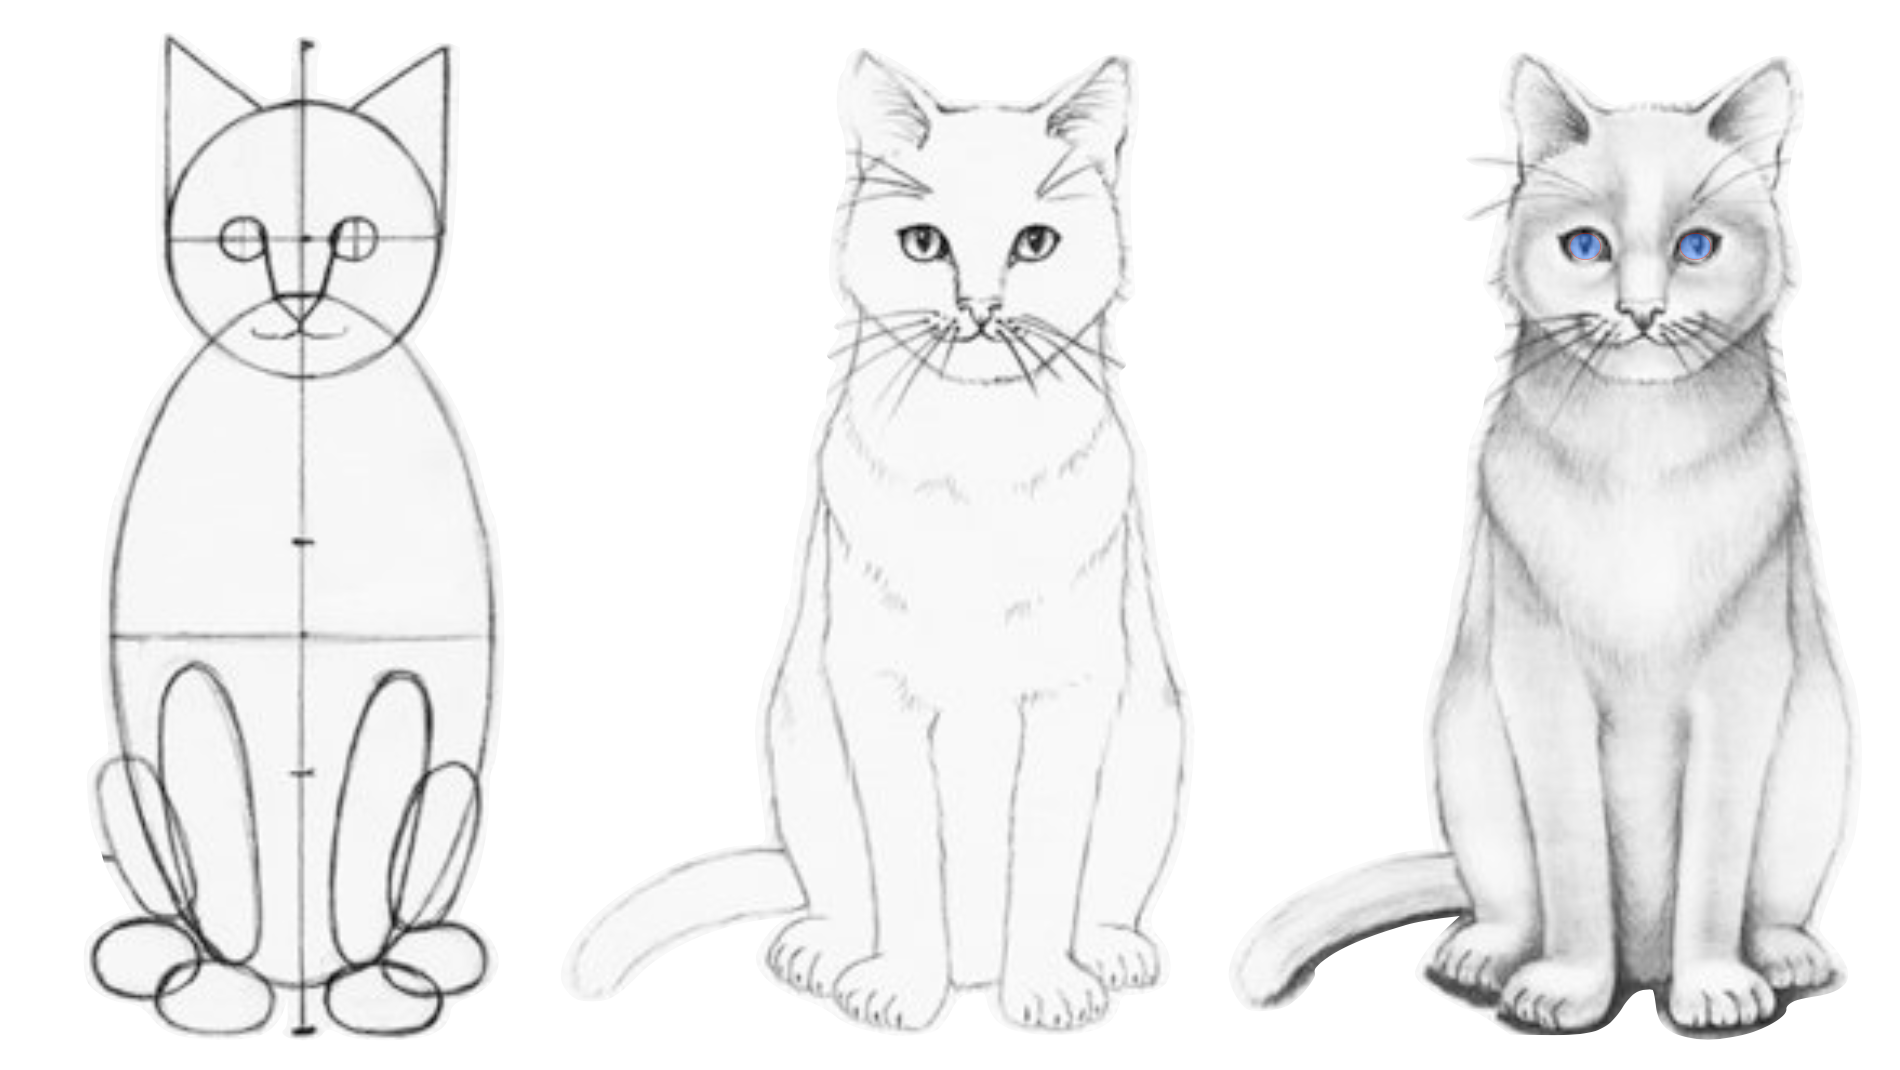
\includegraphics[width=0.35\linewidth]{image10.png}
%     \end{figure}

%     \begin{tcolorbox}[colback=cyan!40, colframe=gray!70, title={The reduced, hierarchical manifold}]
%     \textbf{Hierarchical Constraints}
%     $
%         \mathcal{C}_i(\mathbf{y}_i) = 0
%     $  generate a sequence, $$\mathcal{M}_0 \xrightarrow{\ \mathcal{C}_1\ } \mathcal{M}_1 \xrightarrow{\ \mathcal{C}_2\ } \mathcal{M}_2 \xrightarrow{\ \dots\ } \mathcal{M}_k$$
%     \end{tcolorbox}

% \end{frame}


% %   \begin{frame}{The dimensions of structured experience}
% %   \begin{columns}
% % \begin{column}{0.5\textwidth}
    
% %   During \SEP, the agent's dynamics are confined to a reduced hierarchical manifold.\vspace{0.5cm}
  
% %   The structure of the reduced manifold represents the structure of experience (simplicity aspects, Lie groups). \vspace{0.5cm}
  
% %   Model \textit{accuracy} and \textit{breadth} map into the realism and breadth of experience. \vspace{0.5cm}
  
% % \end{column}
% % \begin{column}{0.5\textwidth}  
% %     \begin{center}
% %          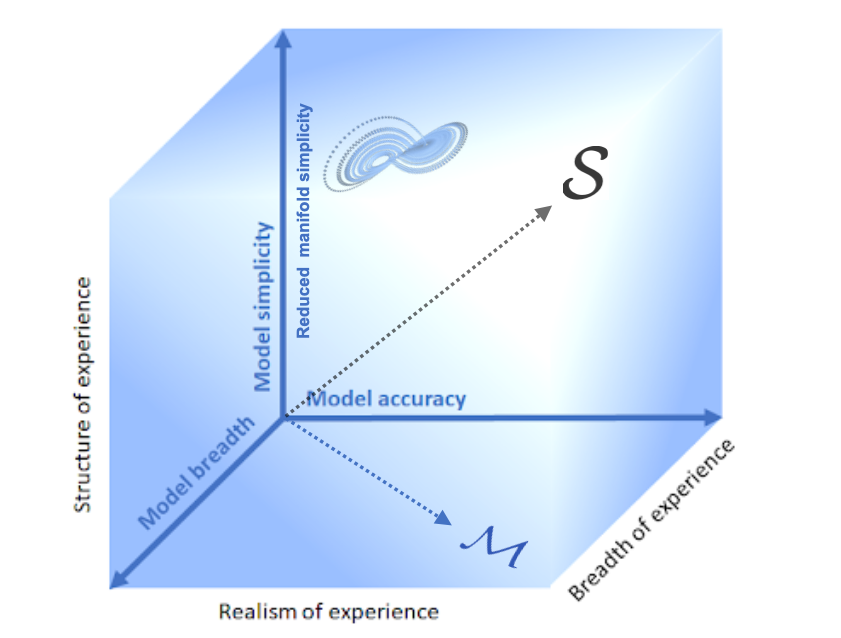
\includegraphics[height=6cm]{img/3dKT2.png}
% %      \end{center}
% % \end{column}
% % \end{columns}

% % \end{frame}
 

% % \begin{frame}[label=ladila]{Summary: Symmetry, dynamics, \K, and \SEP}

% % World-tracking keeps dynamics on the reduced manifold (leading to \SEP!). \vfill 
 
% % The hierarchical reduced manifold is characterized by its structural features (\textbf{symmetry, geometry, topology}). \textbf{This provides the structure in \SEP.}
% % \vfill

% %    \textbf{$\longrightarrow$ Compositional structure in data, the collapse of dynamics to hierarchical manifolds,  criticality,  \K, and \SEP are thus deeply connected.} 

% % \end{frame}

% \begin{frame}[label=summarysymmetry]{Summary: Symmetry, dynamics, \K, and \SEP}

% \begin{itemize}
%     \item World-tracking, symmetry keep dynamics on the reduced manifold, associated with \SEP.
%     \vfill
%     \item The hierarchical reduced manifold is characterized by its structural features (\textbf{symmetry, geometry, topology}).
%     \textbf{This provides the structure in \SEP.}
%     \vfill
% \end{itemize}

% \begin{tcolorbox}[colback=cyan!40, colframe=gray!70, title={Summary}]
%    The compositional structure of world data, the collapse of dynamics to hierarchical manifolds, criticality, \K, and \SEP are deeply connected.
% \end{tcolorbox}

% \end{frame}
